\documentclass{../industrial-development}
\graphicspath{{01-business-processes/}}

\title{Бизнес-процессы компании по разработке программного обеспечения. 
Cхемы организации бизнеса по разработке ПО}
\author{Филонов Дмитрий Русланович}
\date{}

\begin{document}

\begin{frame}
  \titlepage
\end{frame}

\begin{frame}{План лекции}
  \tableofcontents
\end{frame}

\section{Классификация бизнес-процессов}
\subsection{}

\begin{frame} \frametitle{Классификация бизнес-процессов}
По предназначению (характеру деятельности и создаваемому продукту) бизнес-процессы делятся на:
\begin{itemize}
	\item Основные процессы
	\item Вспомогательные процессы
	\item Процессы управления
\end{itemize}
\end{frame}
\lecturenotes
Классификация бизнес-процессов
По предназначению (характеру деятельности и создаваемому продукту) бизнес-процессы делятся на:
\begin{itemize}
	\item Основные процессы
	\item Вспомогательные процессы
	\item Процессы управления
\end{itemize}


\begin{frame} \frametitle{Основные бизнес-процессы}
\begin{itemize}
	\item К ним относят процессы производства, сбыта, снабжения и т.д.
	\item Примеры основных процессов: маркетинг, закупки, производство, хранение, поставка продукции, сервисное обслуживание и другие, связанные с продукцией процессы
\end{itemize}
\begin {block}{Их результат}
Это основной продукт или полуфабрикат для его изготовления.
\end {block}
\end{frame}
\lecturenotes
К \alert{основным} бизнес-процессам относят
\begin{itemize}
	\item Процессы производства, сбыта, снабжения и т.д.
	\item Например, маркетинг, закупки, производство, хранение, поставка продукции, сервисное обслуживание и другие, связанные с продукцией процессы
\end{itemize}


\begin{frame} \frametitle{Вспомогательные бизнес-процессы}
Направлены на обеспечение ресурсов для реализации основных процессов. К ним относят:
\begin{itemize}
	\item Подготовку кадров
	\item Сервисное обслуживание оборудования
	\item Обеспечение связью, IT-обеспечение
	\item Обеспечение безопасности
\end{itemize}
\begin {block}{Важное свойство:}
Деятельность \alert{вспомогательных} бизнес-процессов не касается основных продуктов.
\end {block}
\end{frame}
\lecturenotes
\alert{Вспомогательные бизнес-процессы} направлены на обеспечение ресурсов для реализации основных процессов. 
К ним относят:
\begin{itemize}
	\item Подготовку кадров
	\item Сервисное обслуживание оборудования
	\item Обеспечение связью, IT-обеспечение
	\item Обеспечение безопасности
\end{itemize}
\begin {block}{Важное свойство:}
Деятельность \alert{вспомогательных} бизнес-процессов не касается основных продуктов.
\end {block}


\begin{frame} \frametitle{Процессы управления}
Обеспечивают управление деятельностью компании, регулируют её основные и поддерживающие бизнес-процессы.
\begin{itemize}
	\item Стратегическое управление
	\item Управление финансами 
	\item Управление персоналом
\end{itemize}
\begin {block}{Результат:}
Слаженная и направленная деятельность всей организации.
\end {block}
\end{frame}
\lecturnotes
\alert{Процессы управления} обеспечивают, как не странно, \alert{управление}  деятельностью компании, регулируют её основные и поддерживающие бизнес-процессы.
Некоторые процессы управления:
\begin{itemize}
	\item Стратегическое управление
	\item Управление финансами 
	\item Управление персоналом
\end{itemize}

\begin{frame} 
\begin{block}{}
Рассмотрим как реализуются ранее упомянутые бизнес-процессы в компаниях, разрабатывающих ПО.
\end{block}
\end{frame}

\lecturenotes

\section{Основные бизнес-процессы компании по разработке ПО}

\begin{frame} \frametitle{Основные бизнес-процессы компании по разработке ПО}
Независимо от организации бизнеса:
\begin{itemize}
	\item Разрабатка собственного продукта
	\item Разрабатка под заказ
	\item Аутсорсинг
\end{itemize}
можно выделить \alert{основные} бизнес-процессы ИТ-компаний по разработке ПО. 
\begin {block}{}
Они опираются на определение \alert{жизненного цикла разработки ПО}.
\end {block}
\end{frame}
\lecturenotes
Независимо от выбора методологии разработки ПО или организации бизнеса (компания разрабатывает свой продукт или разрабатывает под заказ) выделяются некоторые основные бизнес-процессы по разработке ПО. Они являются основными, т.к. опираются на определение жизненного цикла разработки ПО.

\begin{frame} \frametitle{Жизненный цикл разработки ПО}
\begin{itemize}

	\item \textbf{Жизненный цикл разработки программного обеспечения} (SDLC---Software Development Life Cycle) - это серия этапов, через которые программное обеспечение должно пройти от своей \textit{концептуализации} до \textit{бесперебойной работы}.

	\item Среди них выделяют технико-экономическое обоснование, проектирование, программирование, тестирование, развертывание, обслуживание и др.
	
\end{itemize}
%\centerline{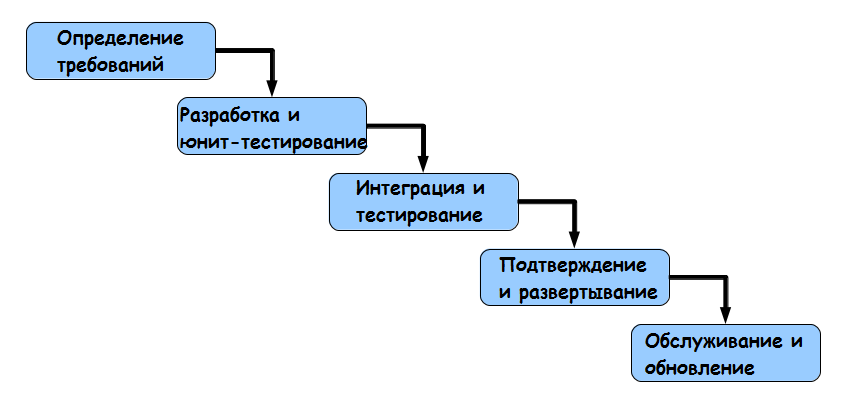
\includegraphics[height=0.6\textheight]{w1.png}}
\end{frame}
\lecturenotes
Жизненный цикл разработки программного обеспечения (SDLC---Software Development Life Cycle) - это серия этапов, через которые программное обеспечение должно пройти от своей концептуализации до бесперебойной работы. Он состоит из всех этапов, необходимых для обеспечения разработки полезного и надежного программного продукта и включают в себя процессы, которые являются экономически эффективными и прослеживаемыми.
SDLC состоит из логически упорядоченных этапов (фаз). Каждая фаза на практике реализуется своим бизнесс-процессом, которые в свою очередь могут делиться на под-процессы~\cite{SDLC}.


\begin{frame} \frametitle{Технико-экономическое обоснование}
После принятия бизнес-заявки:
\begin{itemize}
	\item Определяется объем и содержание проекта
	\item Определяется рентабельность инвестиций (ROI)
	\item Проводится анализ рисков, планирование бюджетирования
	\item Решается главный вопрос проекта---<<Быть или не быть>>
\end{itemize}
\centerline{
\includegraphics[height=0.50\textheight]{g.png}}
\end{frame}
\lecturenotes
Технико-экономическое обоснование:
Это очень важный этап. После принятия бизнес-заявки важно определить объем и содержание проекта. Для определения рентабельности инвестиций (ROI) необходимо провести анализ затрат и выгод, эффективное использование ресурсов, работоспособность и соответствие требованиям клиентов. Результаты этого исследования представлены высшему руководству, что помогает им решить, следует ли продолжать проект. На этом этапе происходит инициирование проекта, его планирование и бюджетирование. Часто бывает полезным перечислить бизнес-требования верхнего уровня на этом этапе в качестве справочного руководства для последующих этапов, а также получить более качественные данные для фактической осуществимости проекта~\cite{SDLC}.

\begin{frame} \frametitle{Сбор и анализ требований}
Описываются детали бизнес-требований верхнего уровня
\begin{itemize}
  \item Клиент разъясняет свои требования
	\item В дополнение к указанным ранее фундаментальным требованиям определяются \alert{производные и неявные}.
	\item Требования могут отображаться через инциденты/сценарии
	\item Происходит согласование команды разработки
\end{itemize}
\begin{block}{Спецификация}
Важный артефакт данного этапа. 
\end{block}
\end{frame}
\lecturenotes
Сбор и анализ требований:
Здесь описываются детали бизнес-требований верхнего уровня. В дополнение к указанным пользователями фундаментальным требованиям необходимо  определить производные и неявные требования. Этот этап важен для разъяснения ожиданий клиента команде разработчиков. Это влечет за собой подробные обсуждения с системными архитекторами, руководителями проектов и конечными пользователями / клиентами. Требования должны быть задокументированы в таком формате, что команда разработки ПО могла её легко понять. Часто используется анализ прецедентов, чтобы отобразить основанное на сценарии сопоставление требований с соответствующим поведением системы.  Важным артефактом данного этапа является спецификация---документ, который точно, полностью и в поддающейся проверке форме определяет требования, устройство, поведение или другие особенности системы, компонента, продукта или услуги~\cite{SDLC}.


\begin{frame} \frametitle{Проектирование (Design)}
Команда разработки решает следующие вопросы
\begin{itemize}
  \item Разбиение спецификации на подзадачи
	\item Определяется архитектура проекта (Design). Она может определяться следующими описаниями:
	\begin{itemize}
		\item HLD (High Level Design)---глобальное описание  проекта
		\item LLD (Low Level Design)---подробное описание его частей
	\end{itemize}
\end{itemize}
\end{frame}
\begin{frame} \frametitle{Проектирование (Design)}
На этапе проектирования также определяются
\begin{itemize}
	\item Аппаратная и программная платформа разработки
	\item Язык программирования
	\item Кадровые и квалификационные требования
	\item Указываются входные и выходные данные, их структура, способ хранения, интерфейсы, процесс управления ПО
\end{itemize}
\end{frame}
\lecturenotes
Разработка:
Системные архитекторы, ведущие разработчики и технические руководители сопоставляют спецификации требований с планом разработки. Часто есть два этапа этой фазы - HLD (High Level Design) и LLD (Low Level Design). Часто используются такие методы, как Data Flow Diagram (диаграммы потока данных), словарь данных, блок-схемы, дерево решений, альтернативный анализ стратегии проектирования. Определяются необходимая аппаратная и программная платформа разработки, язык программирования, кадровые и квалификационные требования для разработки проекта. Указываются входы, выходы, базы данных, структуры данных, интерфейсы, документация и процесс управления программным обеспечением. В этой фазе также проводится анализ рисков~\cite{SDLC}.


\begin{frame} \frametitle{Программирование и юнит (модульное) тестирование (CUT---Coding and Unit Testing)}
\begin{itemize}
\item Построение работающего ПО в соответствии с дизайном разработчиков (HLD, LLD)
\item Каждый программный модуль (юнит) проходит тестирование
\item Программный код должен обладать свойством расширяемости (т.е. предусматривает возможность внесения изменений в дальнейшей разработке)
\item Расширение происходит до тех пор, пока не удовлетворит тестам, определяемых спецификацией или требованиями заказчика 
\end{itemize}
\end{frame}
\lecturenotes
Программирование и юнит (модульное) тестирование (CUT---Coding and Unit Testing) :
Этот этап включает в себя фактическое построение работающего ПО в соответствии с дизайном разработчиков, используя программные и аппаратные платформы на языке программирования, заданном разработчиками системы. Код, разработанный командой проверяется юнит-тестами, чтобы обеспечить обнаружение и удаление любых локальных ошибок. Разработанные программы должны управлять перемещением данных в соответствии с требованиями проекта. Иногда разработчику приходится работать в тесной координации с системными архитекторами, тестировщиками или даже представителями заказчика, так как на любом из этапов может потребоваться переработка, если результаты юнит-тестирования демонстрирует отклонение от ожиданий. Код должен быть модульным по своему характеру и, как правило, должен расширяться в будущем, чтобы избежать существенного исправления при последующем обновлении. Тестовые примеры существуют независимо от кода,  руководствуясь лишь планом тестирования для максимальной эффективности. Ошибки, обнаруженные на этапе юнит-тестирования, более эффективны с точки зрения затрат, чем те, которые были найдены на более поздних этапах~\cite{SDLC}.


\begin{frame}\frametitle{Интеграция и тестирование системы}
\centerline{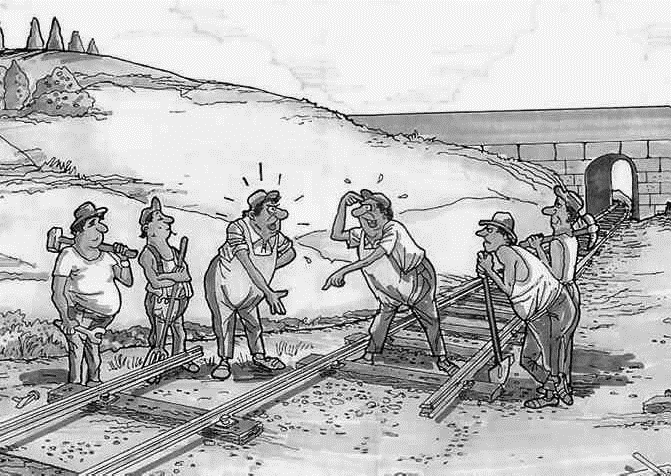
\includegraphics[height=0.5\textheight]{it.png}}
\begin{itemize}
\item Модули (юниты) объединяются
\item Происходит тестирование интегрированного интерфейса и взаимодействие согласно определенной ранее спецификации
\item Обнаруженные ошибки документируются и отправляются  на переработку
\end{itemize}
\end{frame}
\lecturenotes
Интеграция и тестирование системы:
Модули, поставляемые с этапа CUT, объединяются и тестируются их интерфейсы, а также поведение интегрированного программного обеспечения. На этом этапе можно провести различные уровни тестирования. Тестирование интерфейса может проверять поток информации по интерфейсам между модулями. Pair-Wise-Integration (PWI) включает в себя проверку целостности двух взаимодействующих модулей. Системная интеграция подразумевает объединение всех модулей в тестовую среду и тестирование всей системы. Для проведения различных уровней тестирования необходимы хорошие планы испытаний и различные экспертные навыки. Входные данные для планов тестирования, как правило, являются спецификацией требований и проектами, чтобы сохранить ее независимо от перспективы кодирования. Обнаруженные ошибки документируются и отправляются разработчикам для исправления в зависимости от того, где может возникнуть происхождение ошибки. Обновленное программное обеспечение повторно протестировано и подготовлены тестовые отчеты~\cite{SDLC}.


\begin{frame} \frametitle{Внедрение (развертывание/миграция)}
\begin{itemize}
\item Проект на данной стадии должен максимально соответствовать спецификации
\item Перед развертыванием на стороне клиента возможно тестирование продукта его пользователями
\item Проект все еще можно доработать, внеся новые поправки в спецификацию
\item Развертывание может происходить как сразу, так и постепенно (например, когда происходит поверх старой системы)
\item Конец внедрения заканчивается на фазе окончательного перехода от старой системы к новой.
\end{itemize}
\end{frame}
\lecturenotes
Внедрение (развертывание / миграция):
Как только система будет найдена без ошибок, она будет готова к развертыванию на сервере клиента. Перед развертыванием может потребоваться тестирование самими пользователями (владельцами продукта). Документация пользователя в данном случае является важнейшим достижением для этой фазы. Обучение пользователей и ИТ-персонала также может быть частью этого этапа. Развертывание может происходить постепенно, особенно если оно происходит поверх старой системы. Конец внедрения заканчивается на фазе окончательного перехода от старой системы к новой~\cite{SDLC}.

\begin{frame} \frametitle{Обслуживание и обновление}
Эта стадия обеспечивает:
\begin{itemize}
\item Бесперебойную работу в режиме реального времени
\item Исправление непредсказанных на этапе разработки ошибок
\item Оптимизацию приложения
\item Происходит пока ПО или оборудование заказчика не устареет.
\end{itemize}
\end{frame}
\lecturenotes
Обслуживание и обновление:
После развертывания системы ее необходимо поддерживать. Это должно обеспечить бесперебойную работу в среде реального времени. Любые ошибки, обнаруженные во время работы программного обеспечения, должны быть исправлены. На этом этапе необходимо разработать любые дополнительные усовершенствования и дополнительные функции. Крайне важно, чтобы любые изменения, внесенные в запущенную систему, не влияли на производительность системы. Техническое обслуживание программного обеспечения обычно длится до тех пор, пока не устареет или же по истечению контракта~\cite{SDLC}.

\begin{frame} \frametitle{Закрытие проекта}
Этой стадией часто \alert{несправедливо} пренебрегают. Слайдом тоже едва не пренебрегли =) Этап не является обязательным, однако
\begin{itemize}
\item Он может извлечь важные уроки, полученные из опыта разработки 
\item То есть помогает не <<наступить на те же грабли дважды>>
\item Он позволит оптимизировать бизнес-процессы в дальнейшем.
\end{itemize}
\end{frame}
\lecturenotes
Закрытие проекта:
После разработки программного обеспечения хорошо иметь его официальное закрытие, главным образом после того, как были реализованы основные функциональные возможности проекта. На этом этапе важно провести мозговой штурм, чтобы отметить уроки, полученные из проекта, которые могут послужить ценным вкладом в будущие проекты. К сожалению, этот этап часто пропускается, поскольку он не является обязательным, и организации часто не имеют возможности учиться на прошлых ошибках. В результате компания может несколько раз <<наступить на грабли>>, потерять время и увеличить производственные издержки~\cite{SDLC}.
	

\begin{frame} \frametitle{Модели жизненного цикла ПО}
Они также известны как практики/методологии разработки ПО. Их задача---организовать основные бизнес-процессы максимально эффективно. 
\begin{block}{Наибольший контраст проявляется между }  
\begin{itemize}
\item \textbf{Waterfall} (Водопадная модель)
\item \textbf{Agile} (Гибкая методология)
\end{itemize}
\end{block}
\end{frame}
\lecturenotes
Модели жизненного цикла разработки программного обеспечения (SDLC). Также известные как методики/методологии разработки программного обеспечения.
Существует множество таких методик. Наибольший контраст проявляется между Waterfall (Водопадная модель) и Agile (Гибкая метолология).
Модель «Waterfall» использовалась с 80-х годов 20 века. Она является очень формальной и структурированной, требующая тщательного и последовательного выполнения каждого вышеперечисленного бизнес-процесса. Каждая следующая фаза жизненного цикла наступает только после полного завершения предыдущей. Вы получите классическую модель <<Waterfall>>, если последовательно соедините все вышеупомянутые фазы жизненного цикла разработки ПО. Однако, существуют и более гибкие, усовершенствованные версии Waterfall. О них можно узнать, например в труде профессора Winston W. Roуce <<MANAGING THE DEVELOPMENT OF LARGE SOFTWARE SYSTEMS>>~\cite{Winston}.

\begin{frame} \frametitle{Waterfall}
\centerline{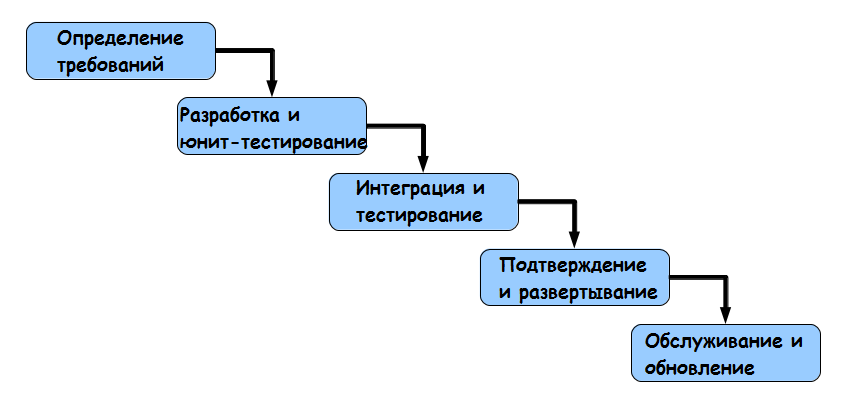
\includegraphics[height=0.6\textheight]{w1.png}}
\end{frame}

\begin{frame} \frametitle{Agile}
\alert{Scrum}---одна из наиболее распространенных Agile практик.
\centerline{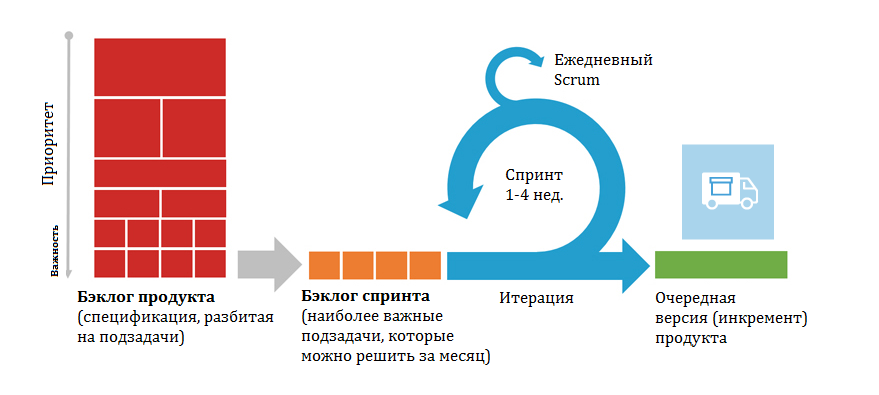
\includegraphics[height=0.6\textheight]{scrum.png}}
\end{frame}
\lecturenotes
Модель Agile была официальна удтвердилась уже в 21 столетии и, как следствие, лучше подстраивается под изменчивые условия внешней среды, позволяя некоторым этапам перекрываться. Модель носит весьма итеративный и нелинейный характер. За счет этого она позволяет максимально сократить издержки и временные простои. 

\begin{frame} \frametitle{Выводы:}
Независимо от 
\begin{itemize}
	\item Вида осуществляемого бизнеса
	\item Предпочитаемых компанией практик
\end{itemize}

выделяются следующие \alert{основные} для разработки ПО бизнес-процессы:
\centerline{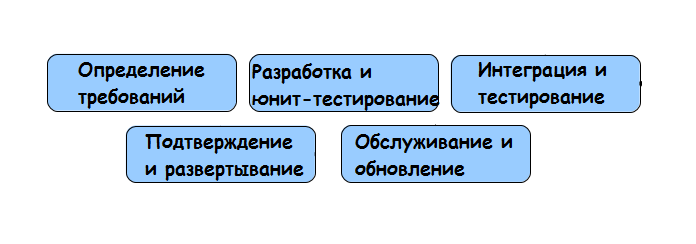
\includegraphics[width=1.35\textheight]{bp1.png}}
\end{frame}
\lecturenotes
В итоге, жизненный цикл разработки программного обеспечения (SDLC) и его правильная организация является ключевым фактором обеспечения получения качественного ПО в контролируемой среде, которая удовлетворяет потребности клиента. 
Независимо от вида осуществляемого бизнеса (осуществляются ли разработка на заказ или передаются на аутсорсинг) и независимо от предпочитаемых компанией практик можно выделить следующие базовые, ключевые для разработки ПО бизнес-процессы: приём заявки на разработку, технико-экономическое обоснование, определение требований, разработка, тестирование, интеграция, развертывание, поддержка и обновление~\cite{SDLC}. Уже взависимости от сложности проекта и распологаемыми компанией ресурсами выбирается методология, определяющая как эти процессы будут взаимодействовать между собой для достижения наилучшего экономического результата.


\begin{frame} \frametitle{Разработка ПО на заказ как \alert{вспомогательный} бизнес-процесс}

\begin {block}{}
Если результат деятельности компании не связан с её основным продуктом, то ИТ-обеспечение является в ней \alert{вспомогательным} бизнес-процессом (они создают условия для реализации основных процессов). ИТ-обеспечение может быть также направлено на оптимизацию процессов управления организацией, например, обучения персонала.
\end {block}
\end{frame}
\lecturenotes
Если результат деятельности компании не связан с её основным продуктом, то ИТ-обеспечение является в ней \alert{вспомогательным} бизнес-процессом (они создают условия для реализации основных процессов). ИТ-обеспечение может быть также направлено на оптимизацию процессов управления организацией, например, обучения персонала.

\begin{frame} \frametitle{Виды корпоративных приложений}
Существует множество различных корпоративных приложений. Их можно классифицировать по доступу: 
\begin{itemize}
		\item Локальные
		\item Облачные
		\item Веб/Мобильные/Кроссплатформенные
\end{itemize}
\end{frame}
\lecturenotes
\alert{Виды корпоративных приложений}
Существует множество различных корпоративных приложений. Их можно классифицировать по доступу: 
\begin{itemize}
		\item Локальные
		\item Облачные
		\item Веб/Мобильные/Кроссплатформенные
\end{itemize}

\begin{frame} \frametitle{Виды корпоративных приложений}
Или по выполняемым функциям:
\begin{itemize}
		\item Для взаимодействия сотрудников и деловых партнеров
		\item Для клиентов и конечных пользователей  
		\item Обслуживание внутренних записей
		\item Управление инфраструктурой
		\item Планирование ресурсов предприятия
		\item Бизнес-аналитика, стратегические альянсы с партнерами
		\item Системы управления контентом
		\item Системы управления обучением 
\end{itemize}
\end{frame}
\lecturenotes
Или по выполняемым функциям:
\begin{itemize}
		\item Для взаимодействия сотрудников и деловых партнеров
		\item Для клиентов и конечных пользователей  
		\item Обслуживание внутренних записей
		\item Управление инфраструктурой
		\item Планирование ресурсов предприятия
		\item Бизнес-аналитика, стратегические альянсы с партнерами
		\item Системы управления контентом
		\item Системы управления обучением 
\end{itemize}
Под заказ ИТ-Компании обычно разрабатывают корпоративные приложения для активного и непосредственного взаимодействия компаний-заказчиков со своими сотрудниками, деловыми партнерами, клиентами и конечными пользователями. Таким образом, программные приложения внесли свой вклад в каждый уровень бизнеса, будь то обслуживание внутренних записей, управление инфраструктурой, планирование ресурсов предприятия, бизнес-аналитика, стратегические альянсы с партнерами, управление взаимоотношениями с клиентами, системы управления контентом, системы управления обучением , или взаимодействия с пользователями или клиентами. Корпоративное приложение может быть создано для эффективного управления ресурсами компании или может позволить локальным работникам получать доступ к данным и инструментам из любого другого места, где расположена их компания. Эти приложения могут быть локальными, веб или облачными.
С появлением множества технологических платформ и устройств стали популярными мобильные приложения. Кроссплатформенность является еще одним важным фактором. Оно позволить приложению работать на нескольких устройствах и, таким образом, снижать общие издержки.
Разработка любого типа приложений требует опыта в конкретных технологиях и понимания тенденций бизнес-требований. Это лучше всего реализовывается путем разработки ПО на заказ под собственные требования. Если бизнес-процессы, связанные с ИТ выходят за рамки разработки ИТ-приложения, то на помощь приходит аутсорсинг. Так, заключив контракт, компания-заказчик сможет частично или полностью передать процессы по поддержке, обслуживанию и модернизации ИТ-инфраструктуры в руки компаний, специализирующихся на абонентском обслуживании организаций и имеющих штат специалистов различной квалификации~\cite{Invensis}. 
\section{Аутсорсинг}


\begin{frame} \frametitle{ИТ-аутсорсинг}
Частичная или полная передача бизнес-процессов ИТ-инфраструктуры в руки компаний, для которых ИТ являются профильным направлением деятельности.
К нему относятся:
\begin{itemize}
	\item Разработка, тестирование и поддержка ПО, информационных систем
	\item Web-хостинг и дизайн
	\item Системная интеграция
\end{itemize}
\end{frame}
\lecturenotes
ИТ-аутсорсинг (англ. IT outsourcing) - частичная или полная передача работ по поддержке, обслуживанию и модернизации ИТ-инфраструктуры в руки компаний, специализирующихся на абонентском обслуживании организаций и имеющих штат специалистов различной квалификации. Для них выполнение подобных работ является профильным направлением деятельности.
ИТ-аутсорсинг предполагает делегирование внешней специализированной компании решения вопросов, связанных с разработкой, внедрением и сопровождением информационных систем, как целиком на уровне инфраструктуры предприятия (сопровождение оборудования или ПО), так и объёмов работ, связанных с развитием и/или поддержкой функционирования отдельных участков системы (программирование, хостинг, тестирование и т.д.)
~\cite[с.~31--38]{Аникин}


\begin{frame} \frametitle{Превосходство аутсорсинга}
Аутсорсинг может способствовать оптимизации \alert{вспомогательных} бизнес-процессов, например, минимизации усилий HR-отдела по найму ИТ-персонала:
\begin{itemize}
		\item Не надо рассматривать каждую кандидатуру по отдельности
		\item Аутсорсинг уже предполагает <<на входе>> готовую, опытную и сложенную команду
		\item Не надо беспокоиться о профессиональном росте сотрудников
\end{itemize}
\end{frame}
\begin{frame} \frametitle{Превосходство аутсорсинга}
Аутсорсинг позволяет
\begin{itemize}
		\item Оптимизировать издержки
		\item Сэкономленные время и финансы могут быть использованы для создания более многофункциональных приложений
\end{itemize}
\end{frame}
\lecturenotes
Почему разработка программного обеспечения для аутсорсинга выгодна?
Усилия, требуемые при найме квалифицированного персонала для разработки собственных приложений, таких как разработчики, технические руководители, руководитель проекта, могут быть довольно утомительными. Более того, поддержание команды и обеспечение регулярного повышения их навыков в соответствии с достижениями в области технологий также являются дорогостоящими. В такой ситуации разработка приложений для аутсорсинга может принести большую пользу, а издержки, сэкономленные в результате, могут быть использованы для создания более многофункционального приложения. ~\cite[с.~31--38]{Аникин}

\begin{frame} \frametitle{Превосходство аутсорсинга}
Аутсорсинговый партнер
\begin{itemize}
		\item уже обладает готовым технический опытом и ресурсами (как трудовые ресурсами, так и инструментами), для разработки приложений
		\item может помочь объективнее воспринимать препятствия и решать их более результативно
		\item может дать консультацию как в рамках одного бизнес-процесса (\alert{ИТ-консалтинг}), так и в течение всего потока процессов.  
		\item может поддерживать приложение в долгосрочной перспективе после его успешного развития
\end{itemize}
\end{frame}
\lecturenotes
Аутсорсинговый партнер по разработке приложений обладает следуищими преимуществами:
\begin{itemize}
	\item Он уже обладает готовым технический опытом и ресурсами (как трудовые ресурсами, так и инструментами), для разработки приложений
	\item Их дальновидность и опыт могут помочь вам объективнее воспринимать препятствия и решать их более результативно
	\item Вы можете пользоваться услугами эксперта для одного этапа процесса разработки приложений или на всех этапах (ИТ-консалтинг)
	\item Если вы смотрите на долгосрочное партнерство, поставщик может поддерживать приложение в долгосрочной перспективе после его успешного развития~\cite[с.~45--54]{Аникин}
\end{itemize}


\begin{frame} \frametitle{Офшорное программирование}
\begin{block}{}
Одна из форм аутсорсинга, предполагающая передачу некритичных для бизнеса процессов (например, \alert{программирования}, которое подразумевает под собой все основные основные бизнес-процессы разработки) компаниям, находящимся в географическом удалении.
\end{block}
При этом:
\begin{itemize}
	\item физическое расположение значения \alert{не имеет}
	\item значение имеет \alert{разный уровень оплаты труда}
\end{itemize}
Выделяются также офшорное тестирование ПО и электронный бизнес.
\end{frame}

\begin{frame} \frametitle{Офшорное программирование}
\begin{itemize}
	\item Мировыми лидерами в сфере Офшорного программирования являются Индия и Ирландия. 
	\item На долю Восточной Европы (включая Россию) приходится около 1 процента рынка (2007)
\end{itemize}
\centerline{
\includegraphics[height=0.6\textheight]{ayre.png}}
\end{frame}

\lecturenotes
Одна из форм ИТ-аутсорсинга, предполагающая передачу некритичных (\alert{вспомогательных}) для бизнеса процессов (например, \alert{программирование}, которое подразумевает под собой все основные основные бизнес-процессы разработки) компаниям, находящимся в географическом удалении. Иными словами — это взаимовыгодное сотрудничество компаний, при котором физическое расположение офисов каждой из них не имеет значения. Наиболее значимой при этом является экономия за счет разного уровня оплаты труда.  ~\cite[с.~76--84]{Аникин}


\begin{frame} \frametitle{Офшорный аутсорсинг}
Помимо разработки программного обеспечения на заказ на аутсорсинг можно вынести
\begin{itemize}
	\item Вспомогательные бизнес-процессы (обеспечение связью, ИТ-обеспечение)
	\item Другие некритичные для бизнеса процессов, требующих большого объема относительно \alert{неквалифицированного} труда 
\end{itemize}
\end{frame}

\lectuenotes
Выделяют следующие разновидности офшорного аутсорсинга:
\begin{itemize}
\item Разработка программного обеспечения на заказ 
\item Вынос второстепенных служб поддержки инфраструктуры 
\item Вынос некритичных для бизнеса процессов, требующих большого объема относительно неквалифицированного труда~\cite[с.~76--84]{Аникин}
\end{itemize}

\begin{frame} \frametitle{Nearshore outsorcing}
Деловые отношения такого рода можно проиллюстрировать на примере стран Северной и Латинской Америки, так как
\begin{itemize}
	\item они находятся на относительно близком географическом расстоянии
	\item расположены примерно в одном часовом поясе
\end{itemize}
\end{frame}
\begin{block} Эти факторы позволяют рационально и в реальном времени совмещать различные бизнес-процессы, в том числе и ИТ-аутсорсинг. \end{block}
\lecturenotes
Офшорное программирование — разработка программного обеспечения для иностранных заказчиков, одна из форм Офшорного аутсорсинга (Offshore outsourcing). Мировыми лидерами в сфере Офшорного программирования являются Индия и Ирландия. На долю Восточной Европы (включая Россию) приходится около 1 процента рынка. Информация взята из Вестника McKinsey, № 17, 2007 г., авторы исследования--- М.Квецински, П.Петерс, Д.Хох прогнозировали рост рынка оффшорного программирования в Восточной и Центральной Европе ~\cite{OutsourceStat}. 
В противовес офшорному аутсорсинга также выделяют Nearshore outsourcing. Деловые отношения такого рода можно проиллюстрировать на примере стран Северной и Латинской Америки, так как они находятся на относительно близком географическом расстоянии и расположены примерно в одном часовом поясе, что позволяет рационально и в реальном времени совмещать различные бизнес-процессы, в том числе и ИТ-аутсорсинг.~\cite{Nearshoring}. 


\section{ИТ-консалтинг}

\begin{frame} \frametitle{ИТ-консалтинг}
\begin{block}{}
\alert{ИТ-консалтинг}  (англ. IT-consulting) — консалтинг в сфере информационных технологий (ИТ). Является одним из многочисленных направлений консалтинга (консалтинговых услуг).
\end{block}
Обычно используется в необходимости
\begin{itemize}
	\item получить независимую экспертную оценку эффективности использования ИТ (обычно в узком спектре, например, защита от DDOS атак)
	\item оптимизировать бизнес-процессы, использующие ИТ
\end{itemize}
\end{frame}
\lecturenotes 
ИТ-консалтинг (англ. IT-consulting) — консалтинг в сфере информационных технологий (ИТ). Является одним из многочисленных направлений консалтинга (консалтинговых услуг).
ИТ-консалтинг — проектно-ориентированная деятельность, связанная с информационной поддержкой бизнес-процессов, позволяющая дать независимую экспертную оценку эффективности использования информационных технологий.
На сегодняшний день большинство компаний использует ИТ в управлении своим бизнесом. Информационные технологии позволяют делать бизнес более наглядным, более управляемым, более прогнозируемым.
ИТ-консалтинг — это услуга, которую предлагают ИТ-компании (как правило в вопросах комплексных проектов), а также независимые эксперты в том или ином направлении IT (обычно в узком спектре, например, защита от DDOS атак).



\begin{frame} \frametitle{Когда нужен ИТ-консалтинг?}
\begin{itemize}
	\item Компания нуждается в свежих идеях
	\item Компания нуждается в опыте, знаниях или оценке деятельности
	\item Компания не нуждается в передаче \alert{вспомогательных}  бизнес-процессов
	
\end{itemize}
\end{frame}
\lecturenotes
Когда нужен консалтинг?
Компания нуждается в свежих идеях.
Компания нуждается в опыте и знаниях.
В руководстве компании нет согласия по важному вопросу, и требуется мнение извне, чтобы получить объективный совет.
Компании нужна помощь для завершения какого-либо проекта.
Из-за недостатков внутрикорпоративных коммуникаций компании нужен специалист, способный стать связующим звеном между уровнями и подразделениями~\cite[с.~187]{Phelan}.



\begin{frame} \frametitle{Виды услуг в ИТ-консалтинге}
\begin{itemize}
	\item Оптимизация затрат на внедрение информационных технологий, ИТ-решений в рамках компании
	\item Повышение эффективности бизнес-процессов компании
	\item Повышение управляемости, прозрачности деятельности организации за счет создания единой ИТ-инфраструктуры
	\item Внедрение систем уровня предприятия (ERP, CRM, Business Intelligence, Groupware-системы, NIS-системы)
	\item ИТ-аудит (оценка уровня автоматизации)
\end{itemize}
\end{frame}

\lecturenotes
Услуга по предоставлению ИТ-консалтинга, как правило, включает следующие пункты:
\begin{itemize}
	\item Оптимизация затрат на внедрение информационных технологий, ИТ-решений в рамках компании
	\item Повышение эффективности бизнес-процессов компании
	\item Повышение управляемости, прозрачности деятельности организации за счет создания единой ИТ-инфраструктуры
	\item Внедрение систем уровня предприятия (ERP, CRM, Business Intelligence, Groupware-системы, NIS-системы)
	\item ИТ-аудит (оценка уровня автоматизации)
\end{itemize}




\section{Разработка собственного ПО}

\begin{frame} \frametitle{Разработка собственного ПО}
\alert{Основные} бизнес-процессы по разработке ПО остаются неизменными. Но появляется одно
  \begin{block}{Очень важное обстоятельство}
   Не совсем ясно---кто заказчик?\dots
  \end{block}
Компания сама выпускает актуальное по её мнению приложение на рынок. В дальнейшем никто не запрещает ей, например, заключать аутсорсинговые контракты.
\end{frame}

\begin{frame} \frametitle{Разработка собственного ПО}
Отсутствие конкретного заказчика влечет за собой появление дополнительных бизнес-процессов \alert{управления}. Для того, чтобы приложение окупило себя, от компании требуются процессы \alert{формирования стратегии, планирования бизнеса и контроля:}.
\begin{itemize}
	\item Cтратегическое управление 
	\item Управление финансами  
	\item Управление маркетингом
\end{itemize}
\end{frame}
Отсутствие конкретного заказчика влечет за собой появление дополнительных бизнес-процессов на стратегическом уровне. Для того, чтобы приложение окупило себя, требуется 
Иметь на руках отличную идею для приложения, обладающее некоторой ценностью
Разработать бизнес-модель приложения, его метрику и экономику, модель монетизации
Проанализировать рынок, конкурентов и целевую аудиторию
Разработать MVP, 
PR-компанию, привлечь инвестиции и капитал

\begin{frame} \frametitle{Маркетинг}
Для того, чтобы ПО окупило себя, требуется 
\begin{itemize}
	\item Иметь на руках отличную идею для приложения, обладающее некоторой ценностью
	\item Разработать бизнес-модель приложения, его экономику и модель монетизации
	\item Проанализировать рынок, конкурентов и целевую аудиторию
	\item Разработать MVP(продукт минимальной стоимости), PR-компанию, привлечь инвестиции и капитал
\end{itemize}
\end{frame}

\lecturenotes
Главной особенностью разработки собственного ПО является 
отсутствие конкретного заказчика.Это осутствие влечет за собой появление дополнительных бизнес-процессов \alert{управления}. \alert{Основные} производственные процессы остаются неизменными.
Для того, чтобы приложение окупило себя, от компании требуются процессы \alert{формирования стратегии, планирования бизнеса и контроля:}.
\begin{itemize}
	\item Cтратегическое управление 
	\item Управление финансами  
	\item Управление маркетингом
\end{itemize}
Для успешного выхода на рынок требуется 
\begin{itemize}
	\item Иметь на руках отличную идею для приложения, обладающее некоторой ценностью
	\item Разработать бизнес-модель приложения, его экономику и модель монетизации
	\item Проанализировать рынок, конкурентов и целевую аудиторию
	\item Разработать MVP(продукт минимальной стоимости), PR-компанию, привлечь инвестиции и капитал~\cite{iidf}
\end{itemize}

Текст конспекта, относящийся к слайду с указанием источника~\cite[с.~97--99]{Brooks}.
На интернет-источники можно ссылаться не по ГОСТу, но с обязательной гиперссылкой~\cite{Fowler}.

\begin{thebibliography}{99}
\bibitem{Phelan} Фелан К. Простите, я разрушил вашу компанию : Почему бизнес-консультанты — это проблема, а не решение = I’m Sorry I Broke Your Company : Why Management Consultants Are the Problem, Not the Solution / Карен Фелан. М~: Альпина Паблишер, 2013. — 224 с. — ISBN 978-5-9614-4463-6.
\bibitem{Winston} \href{http://www.cs.umd.edu/class/spring2003/cmsc838p/Process/waterfall.pdf}{Dr. Winston W. Roуce. MANAGING THE DEVELOPMENT OF LARGE SOFTWARE SYSTEMS}
\bibitem{Аникин} Аникин Б.А. Аутсорсинг: создание высокоэффективных и конкурентоспособных организаций. М.: Инфра-М, 2003. — 192 с. 
\bibitem{Invensis} \href{https://www.invensis.net/blog/it/how-to-outsource-software-app-development/?utm_source=invensis-blog&utm_campaign=blog-post&utm_medium=content-link&utm_term=software-development-life-cycle-phases}
\bibitem{SDLC} \href{https://www.invensis.net/blog/it/software-development-life-cycle-phases/?utm_source=invensis-blog&utm_campaign=blog-post&utm_medium=content-link&utm_term=20-best-practices-for-successful-software-development-projects}
\bibitem{OutsourceStat} \href{http://vestnikmckinsey.ru/operations/skryhtyhj-potencial-autsorsinga-v-vostochnoj-evrope}{Статистика аутсорсинга в Восточной Европе}
\bibitem{Курс <<Интернет-предпринимательство>> ФРИИ} \href{http://iidf-eco.directual.com/#/start}
\bibitem{Nearshoring}\href{https://en.wikipedia.org/wiki/Nearshoring}
\end{thebibliography}

\end{document}

%%% Local Variables: 
%%% mode: TeX-pdf
%%% TeX-master: t
%%% End: 
